\section*{Learning Objectives}

\begin{itemize}
\item In Robotics Engineering, we are constantly faced with problems for which no closed form solution is possible. For such problems, we seek algorithms that compute solutions. In many cases, these algorithms do not terminate with an exact answer in  a finite number of steps. Hence, we need to understand how to formulate and analyze the convergence of iterative processes. 

\item Another class of problems involve maximizing or minimizing real valued functions. It is important to understand sufficient conditions for extrema of real valued functions to exist.


\end{itemize}

\section*{Outcomes} 
\begin{itemize}
\item  Understand the concepts of open and closed sets in normed spaces.
\item Understand sequences and how to analyse if they have limits.
\item Characterize open and closed sets in terms of distance (ie., using the norm directly) and in terms of convergent sequences.
\item Understand in a rigorous manner what is a continuous function. While we saw the definition in Calculus, for most of us, it did not stick!
\item Learn an interesting topological property called compactness and how it relates to the existence of extrema of functions.
\end{itemize}

\newpage



\section{Open and Closed Sets in Normed Spaces} 

We start with a few preliminaries. Let $(\mathcal{X},\ \real,\ \|\bullet\|)$ be a real normed space. Recall from Chapter~\ref{sec:NormsDistance} that a norm is a function $\|\bullet\|:\ \mathcal{X}\to[0,\ +\infty)$ satisfying
    \begin{enumerate}
       \renewcommand{\labelenumi}{(\alph{enumi})}
        \setlength{\itemsep}{.1cm}
        \item $\|x\|\geq 0$ and $\|x\|=0\ \iff\ x=0$
        \item $\|\alpha\cdot x\|=|\alpha|\cdot\|x\|$ for all $\alpha\in\real$, $x\in\mathcal{X}$
        \item $\|x+y\|\leq\|x\|+\|y\|$ for all $x,\ y\in\mathcal{X}$.
    \end{enumerate}
In addition, recall that
    \begin{enumerate}
       \renewcommand{\labelenumi}{(\alph{enumi})}
        \setlength{\itemsep}{.1cm}
        \setcounter{enumi}{3}
        \item For $x,\ y\in\mathcal{X}$, $d(x,\ y):=\|x-y\|$.
        \item For $x\in \mathcal{X}$, $S\subset\mathcal{X}$ a subset, $d(x,\ S):=\inf_{y\in S}\|x-y\|.$
        \item $ A \subset B  \iff A \cap (\sim B) = \emptyset$.
    \end{enumerate}

\begin{definition}Let $x_0\in \mathcal{X}$ and $a\in\real$, $a>0$. The \textbf{ open ball of radius $a$ center at $x_0$} is
    \begin{equation*}
        B_a(x_0)=\{x\in\mathcal{X}~|~\|x-x_0\|<a\}.
    \end{equation*}
    
\end{definition} 

\begin{figure}[hbt!]%
	\centering{
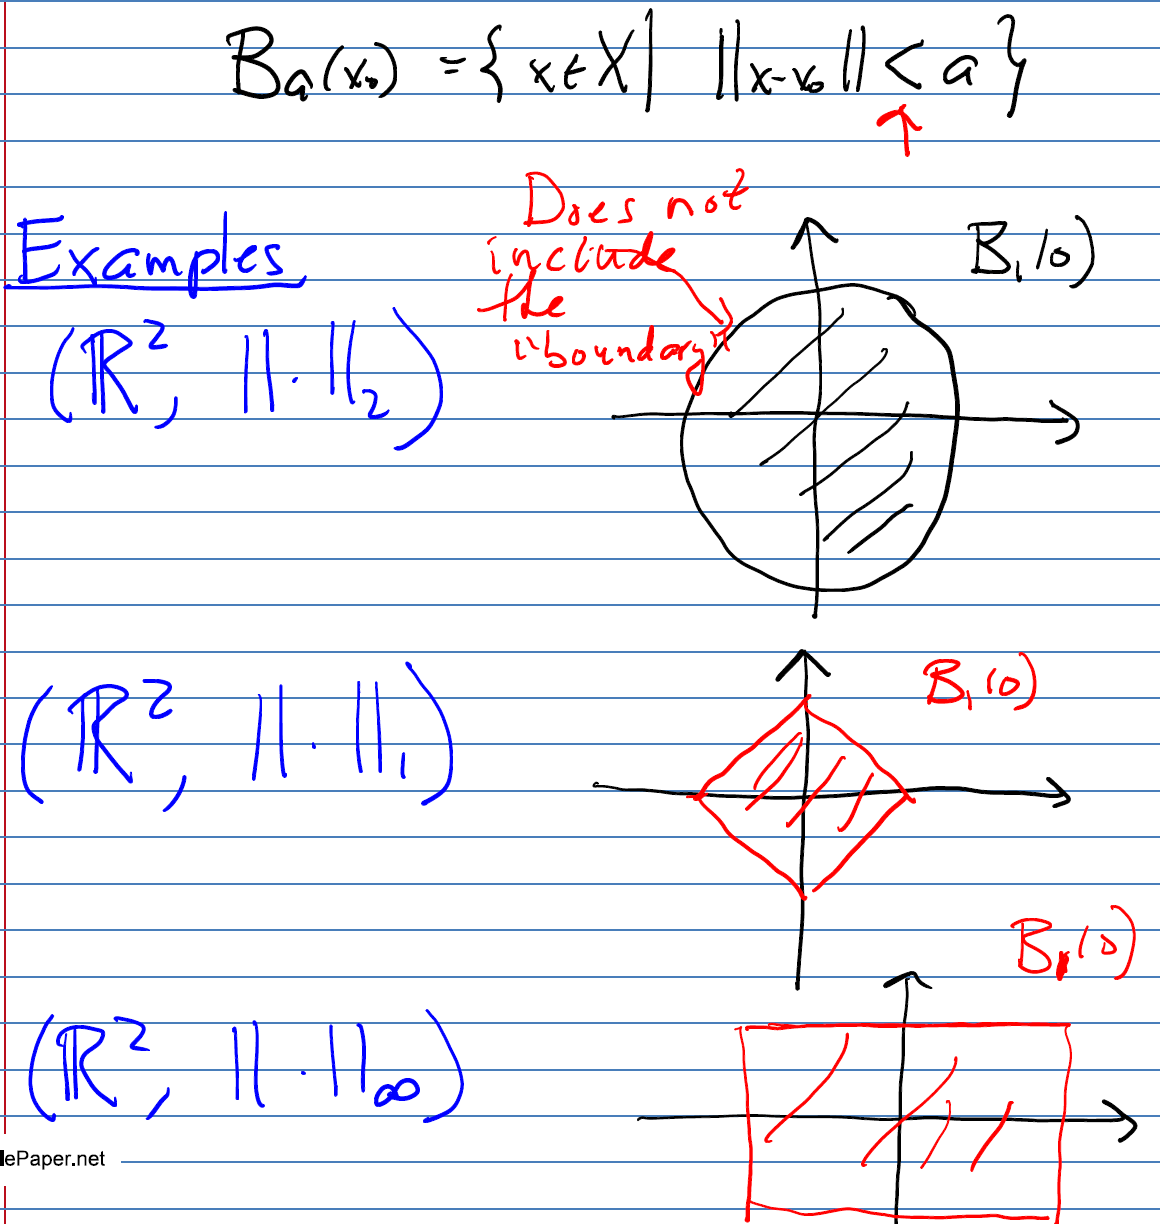
\includegraphics[width=0.7\columnwidth]{graphics/Chap06/UnitBalls.png} }
    \caption[]{ $\left(\real^2,\ \|\bullet\|\right)$ with various norms: (a) Euclidean norm $\|(x_1,\ x_2)\|_2=\sqrt{|x_1|^2+|x_2|^2 }$; (b) One norm  $\|(x_1,\ x_2)\|_1=|x_1|+|x_2|$; and (c) Max norm $ \|(x_1,\ x_2)\|_\infty=\max_{1\leq i\leq 2}|x_i|$. }
    \label{fig:UnitBalls}
\end{figure} 


\begin{lem}\textbnf{(Characterization of distance zero and greater than zero)} Let $\left(\mathcal{X},\ \| \bullet \|\right)$ be a normed space, $x\in\mathcal{X}$, and $S\subset\mathcal{X}$. Then,
    \begin{align*}
        d(x,\ S)=0 &\iff \forall\epsilon>0,\ \exists y\in S,\ \|x-y\|<\epsilon ~~(\text{definition of  the infimum})\\
        &\iff \forall\epsilon>0,\ B_\epsilon(x)\cap S\neq \emptyset ~~(\text{definition of an open ball of radius} ~\epsilon). \text{ Moreover, } \\
        \\
        d(x,\ S)>0 &\iff \exists\epsilon>0,\ \forall y\in S,\ \|x-y\|\geq\epsilon\\
        &\iff \exists\epsilon>0 \textnormal{ such that } B_\epsilon(x)\cap S = \emptyset\\
        &\iff  \exists\epsilon>0 \textnormal{ such that } B_\epsilon(x)\subset (\sim S).
    \end{align*}
\end{lem} 

\begin{figure}[hbt!]%
    \label{fig:DistanceZero2aSet}
\centering{
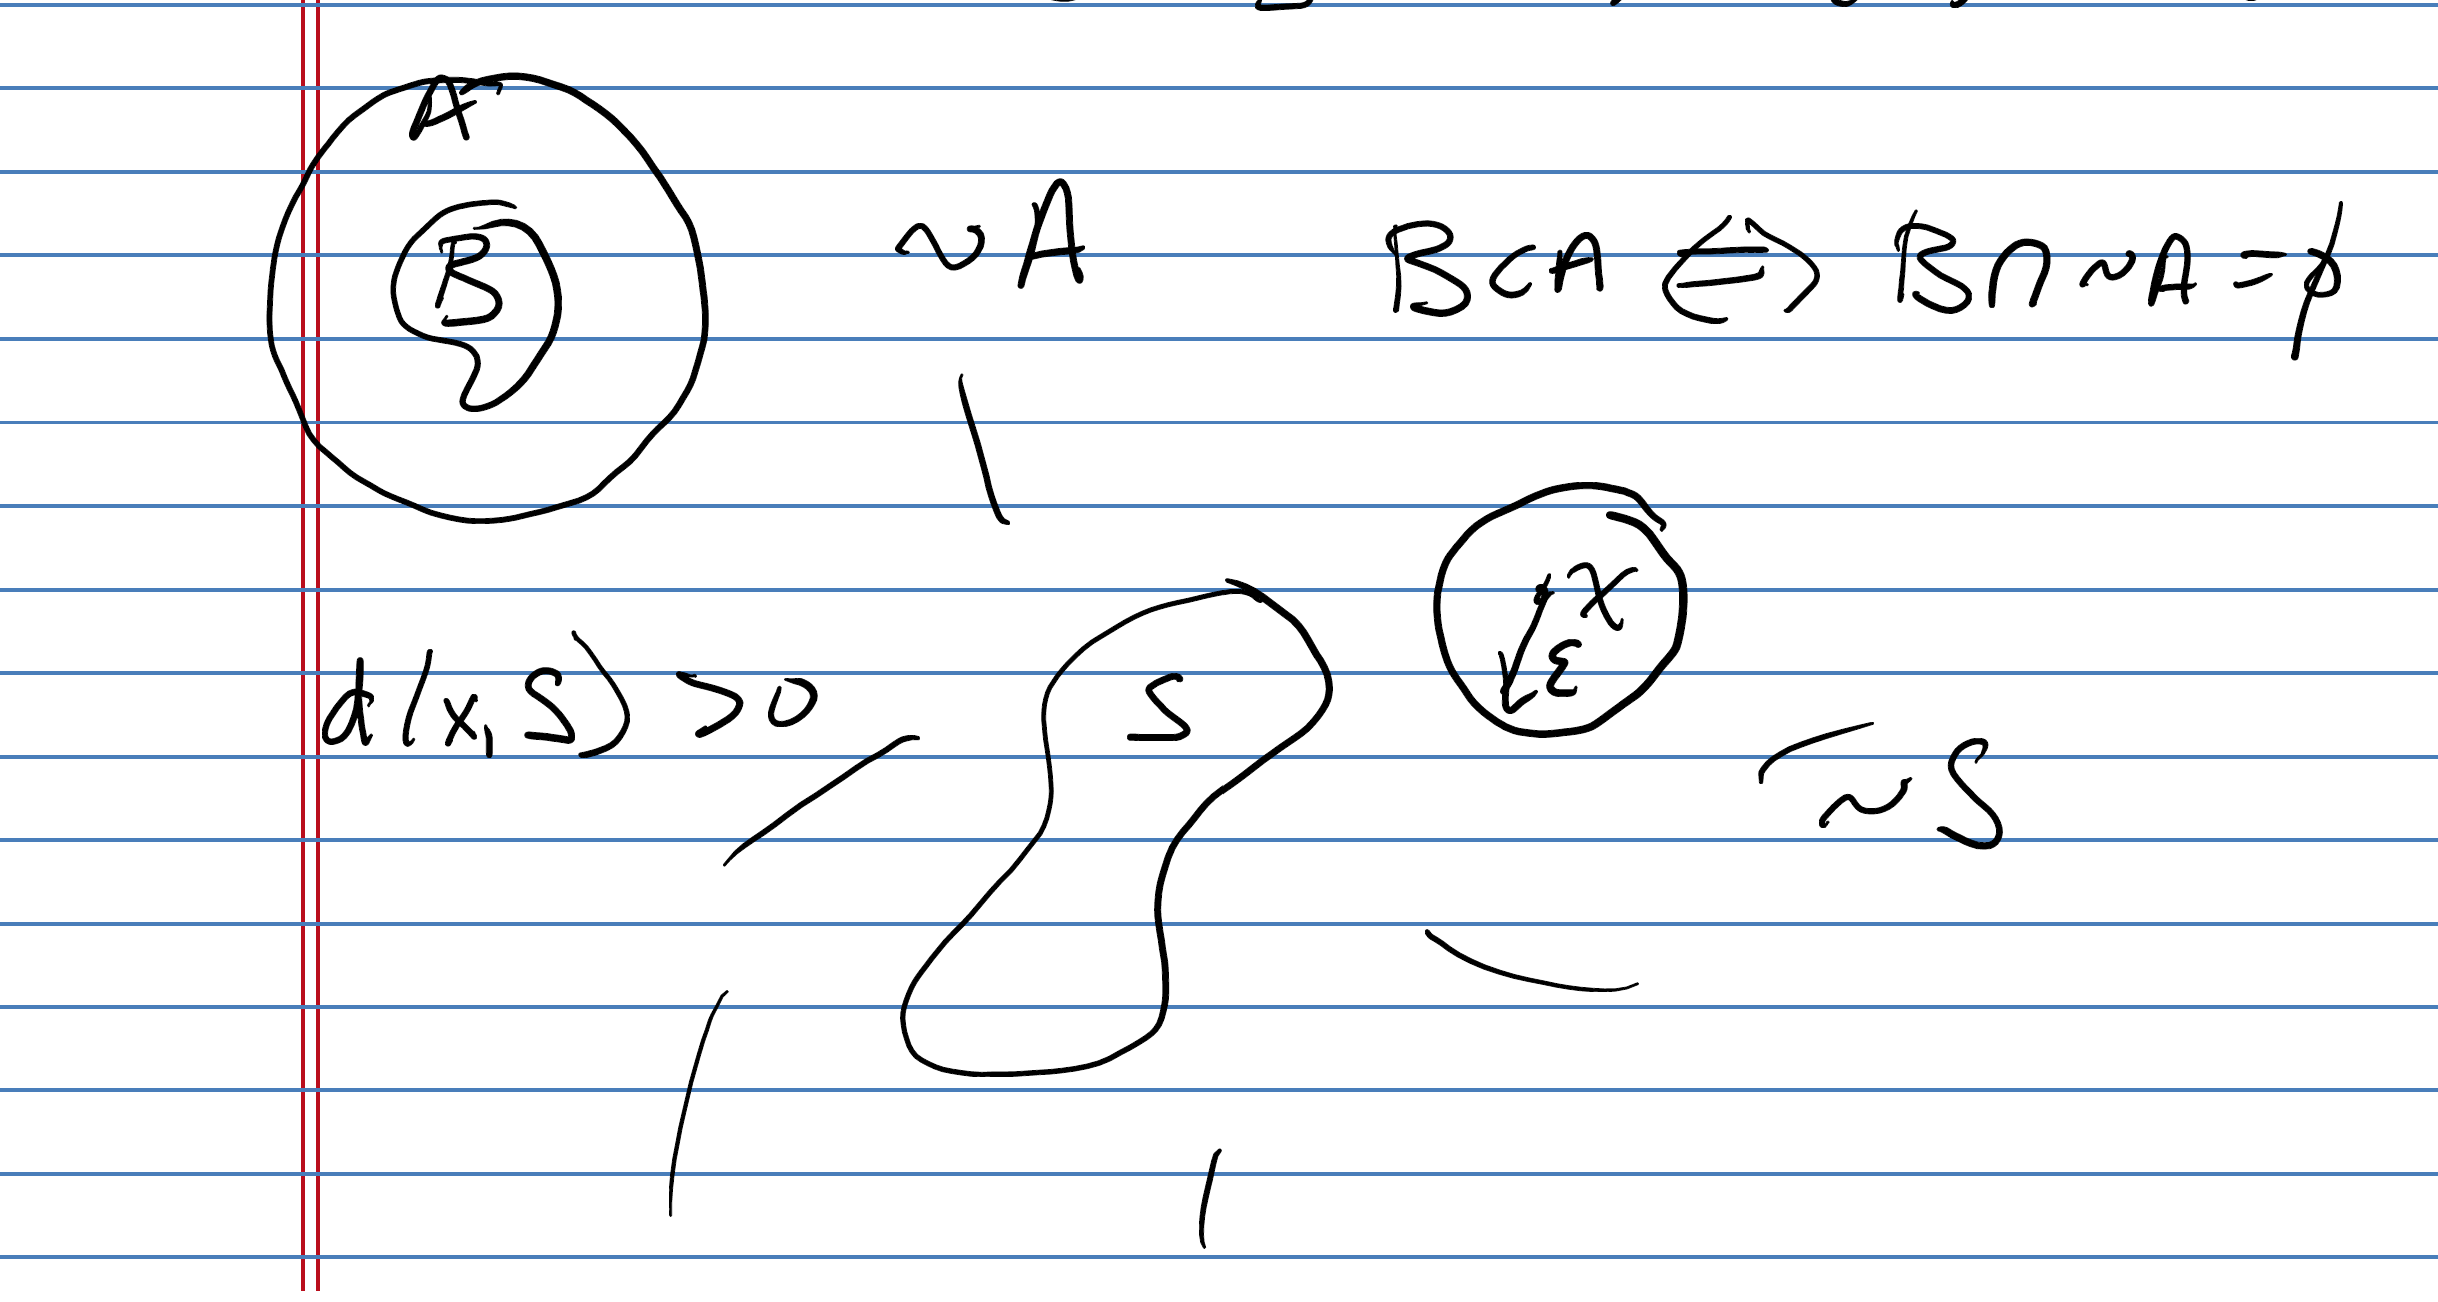
\includegraphics[width=0.7\columnwidth]{graphics/Chap06/DistancextoSpositive.png} 
}
\caption[]{ Why $(d(x, S)>0) \iff (\exists ~\epsilon>0$ such that $ B_\epsilon(x) \subset (\sim S)) \iff (\exists ~\epsilon>0$ such that $ B_\epsilon(x) \cap S = \emptyset)$. We simply take $\epsilon = \frac{d(x, S)}{2} >0.$ }
\end{figure} 


 In the following, we assume $\left(\mathcal{X},\ \| \bullet \|\right)$ is given.
 
\begin{definition} Let $P\subset\mathcal{X}$, a subset of $\mathcal{X}$. 
    \begin{enumerate}
          \renewcommand{\labelenumi}{(\alph{enumi})}
        \setlength{\itemsep}{.1cm} 
        \item A point $p\in P$ is \textbf{ an interior point of $P$} if $\exists\epsilon>0$ such that $B_\epsilon(p)\subset P$.
        \item The \textbf{interior of $P$} is $\mathring{P}:=\{p\in P\ |\ p\textnormal{ is an interior point}\}$.
            \end{enumerate}
\end{definition}

\begin{rem} \mbox{ }
\begin{align*}
    \mathring{P} & = \{ p \in P~ |~ \exists \epsilon >0, B_\epsilon(p) \subset P\} \\
        & = \{ p \in P~ |~ d(p, \sim P) >0\} \\
        & =  \{ x \in \mathcal{X}~ |~ d(x, \sim P) >0\}
\end{align*}
because if $x \in (\sim P)$, then $d(x, \sim P)=0$ and $\mathcal{X} = P \cup (\sim P)$. Hence, 
\begin{center}
 $$ \boxed{\mathring{P} = \{ x \in \mathcal{X}~|~ d(x, \sim P) > 0 \}.}$$
\end{center}
\end{rem}

\begin{definition} $P$ is \textbf{open} if $\mathring{P} =P$.
\end{definition}

\begin{rem} Hence, $P$ is open if, and only if, $P= \{ x \in \mathcal{X}~|~ d(x, \sim P) > 0 \}$.

\end{rem}
    

\begin{example} Checking if sets are open or not.
\begin{itemize}
        \item Is $P=(0,\ 1)\subset(\real,\ \| \bullet \|)$ open? We note that $(x \in P \implies  0 < x < 1)$ and define $\epsilon = \min\{\frac{x}{2}, \frac{1-x}{2}\} $. Then $B_\epsilon(x) \subset P$ and hence $P$ is open.\\
        
        \item  Is $P=(0,\ 1)\subset(\real,\ \| \bullet \|)$ open? We check it a second  way. $\sim P = (-\infty, 0] \cup [1, \infty)$. We have $x \in P \iff 0 < x < 1$. Hence, 
        \begin{align*}
                d(x, (-\infty, 0])&=x>0\\
                d(x,  [1, \infty))&=1-x>0\\
                d(x, \sim P) &= \min\{x, 1-x\} > 0.
        \end{align*}
            Hence, $x \in P \iff d(x, \sim P) >0$, and thus $P$ is open.
        \item $P=[0,\ 1)\subset(\real,\ |  \bullet |)$ is not open because $0\in P$, and $\forall\epsilon>0$, $B_\epsilon(0)\cap(\sim P)\neq\emptyset$ or we can also check it's not open because $0\in P$ and $d(0, \sim P)=0$.
    \end{itemize}

    
\end{example}
    
\begin{definition} $P\subset \mathcal{X}$ a subset.
\begin{enumerate}
        \item A point $x\in \mathcal{X}$ is a \textbf{closure point} of $P$ if $\forall\epsilon>0$, $\exists p\in P$ such that $\|x-p\|<\epsilon$, in other words,  $d(x, P)=0$.
        \item The \textbf{closure of} $P$ is $\overline{P}:=\{x\in\mathcal{X} ~|~ x \text{ is a closure point}\}$
    \end{enumerate}
\end{definition}

\begin{definition}  $P$ is \textbf{closed} if $\overline{P}=P$.

\end{definition}
    

\begin{example} Consider $(\mathcal{X}, \| \bullet \|) = (\real,| \bullet |). $
    \begin{enumerate}
    \item $P=[0,\ 1)$ is not closed because $1 \not \in P$, and $d(1,P)=0$.
    \item $P=[0,\ 1]$ is closed because $x \not \in P$ implies $d(x, P)=\max\{-x, x-1  \} >0$.
        \item $P=(0,\ 1)\implies \overline{P}=[0,\ 1]$ because $d(0, P)=0$, $d(1, P)=0$ and for $x\not \in [0, 1], d(x, P)>0$.
    \end{enumerate}
\end{example}

\begin{fact} The rational numbers $\mathcal{Q} \subset \real$ are neither closed nor open. $\overline{\mathcal{Q}}=\real$.
    
\end{fact}
    


\begin{thm} \textbf{(Characterization of Open and Closed Sets using Distance)} Let $(\mathcal{X}, \| \bullet \|) $ be a normed space and $P\subset \mathcal{X}$ a subset. Then $P$ is open if, and only if, $\sim P$ is closed. \\
\begin{center}
\boxed{
\begin{aligned}
        P\textnormal{ is closed}&\iff\ \sim P\textnormal{ is open}.\\
        P\textnormal{ is open} &\iff\ \sim P\textnormal{ is closed}.
    \end{aligned}
}
\end{center}
  \end{thm}
   

\textbf{Proof:} The proof can be given in one line.
$$\boxed{
    \underbrace{\sim P=\sim(\mathring{P})}_{P\textnormal{ is open}}=\{x\in\mathcal{X}\ |\ d(x,\ \sim P)=0\}=\underbrace{\overline{\sim P}=\sim P}_{\sim P\textnormal{ is closed}}
    }
$$
We'll unpack it for you. 

\begin{align*}
    P = \mathring{P} & \iff P = \{ x \in \mathcal{X}~|~ d(x, \sim P) > 0 \}\\
                        & \iff P = \{ x \in \mathcal{X}~|~\exists \epsilon >0, B_\epsilon(x) \cap P = \emptyset\}\\
                      &  \iff P = \sim \{ x \in \mathcal{X}~|~\forall \epsilon >0, B_\epsilon(x) \cap P \neq \emptyset\}\\
                       &  \iff \sim P = \{ x \in \mathcal{X}~|~\forall \epsilon >0, B_\epsilon(x) \cap P \neq \emptyset\}\\
                       &  \iff \sim P = \{ x \in \mathcal{X}~|~d(x, \sim P) = 0\}\\
                       &  \iff \sim P = \overline{\sim P}
\end{align*}
Hence, $P = \mathring{P} \iff \sim P = \overline{\sim P}$, so $P$ is open if, and only if, $\sim P$ is closed. 
\Qed
 \begin{rem} Can a set be both open and closed? Yes. Such sets are sometimes called \textbf{clopen}! If $(\mathcal{X}, \| \bullet \|)$ is a normed space, then $\mathcal{X}$ is both open and closed. By convention,the empty set $\emptyset$ is both open and closed (Why? For two reasons: (i) Because it does not violate the conditions to be open or closed. (ii) We want the set complement of an open set to be a closed set and vice versa). 
 \end{rem}
 
 \begin{exercise} Show the following:
 \begin{enumerate}
    \renewcommand{\labelenumi}{(\alph{enumi})}
        \setlength{\itemsep}{.1cm}
     \item An arbitrary union of open sets is open.
     \item A arbitrary intersection of closed sets is closed.
     \item A finite intersection of open sets is open.
     \item A finite union of closed sets is closed.
 \end{enumerate}
 \end{exercise}
 
  
 \begin{example} Consider the real numbers as a normed space; that is,  ${\cal X} = \real$ and define the norm to be $||x|| = |x|$, the standard absolute value. Is the infinite intersection of open sets $$ \bigcap\limits_{n=1}^{\infty} (-1- \frac{1}{n}, 1)    $$ open?
 \end{example}
 
 \textbf{Solution:} \textbf{No}. Indeed, $\forall~n\ge 1$, $[-1,1) \subset (-1- \frac{1}{n}, 1)$. Hence, by definition of the intersection, $[-1,1) \subset \bigcap\limits_{n=1}^{\infty} (-1- \frac{1}{n}, 1)$. Moreover, $$[-1,1) = \bigcap\limits_{n=1}^{\infty} (-1- \frac{1}{n}, 1), $$
      because if $x<-1$, then there exits $1\le K<\infty$ such that $x < -1-\frac{1}{K}$, which implies that $x\not \in  (-1- \frac{1}{K}, 1)$, and thus
      $$ x \not \in \bigcap\limits_{n=1}^{\infty} (-1- \frac{1}{n}, 1). $$
      
\Qed
 
 \begin{exercise} Show the following:
  \begin{enumerate}
     \renewcommand{\labelenumi}{(\alph{enumi})}
        \setlength{\itemsep}{.1cm}
     \item $P$ is closed if, and only if, $\overline{P} \subset P$.
     \item $P$ is open if, and only if, $ P \subset \mathring{P}$.
 \end{enumerate}
 
 \end{exercise} 
 
 \begin{definition} The \textbf{boundary} of $S \subset \mathcal{X}$ is $\partial S:= \overline{S} \cap \overline{(\sim S)}.$
 \end{definition}
 
 \begin{exercise} Show that $\partial S= \overline{S} \setminus \mathring{S} := \{ x \in \overline{S}~|~ x \not \in \mathring{S}\}$.
 
 \end{exercise}

\section{Newton-Raphson Algorithm}

As Roboticists and Engineers, we are often faced with problems for which closed-form solutions are unknown or do not exist. For such problems, we often seek iterative means to either compute a solution or to prove the existence of a solution. \\

Consider a function $f:\real^n \to \real^n$ that is continuously differentiable and suppose we seek a root $f(x^\ast)=0$. Note that the domain and range are both $\real^n$ and thus this is the nonlinear equivalent of solving a square linear equation $Ax-b=0$.\\

The \textbf{Newton-Raphson} Algorithm is a vector version of Newton's Algorithm; see Chapter 11 of the ROB 101 Textbook. Let $x_k \in \real^n$ be our current approximation of a root of the function $f$. We write the linear approximation of $f$ about the point $x_k$ as
\begin{equation}
    \label{eq:NewtonMethodVector01}
    f(x) \approx f(x_k) + \frac{\partial f(x_k)}{\partial x}\cdot (x - x_k).
\end{equation}
We want to chose $x_{k+1}$ so that $f(x_{k+1})=0$, but we cannot do that exactly. Based on the linear approximation in \eqref{eq:NewtonMethodVector01}, we have that 
\begin{equation}
    \label{eq:BasicNewtonRaphson}
     f(x_{k+1}) \approx 0 \iff  0  \approx f(x_k) + \frac{\partial f(x_k)}{\partial x}\cdot (x_{k+1} - x_k).
\end{equation}
If $\det\left(\frac{\partial f(x_k)}{\partial x} \right)\neq 0$, we can solve for $x_{k+1}$, giving us the standard form of the Newton-Raphson Algorithm, 
$$ \boxed{    x_{k+1}=x_{k} - \left(   \frac{\partial f(x_k)}{\partial x}\right)^{-1} f(x_k).}$$


The ``hope'' is that each iteration of the algorithm produces a better approximation $x_k$ to a root of the function $f(x)$, where by a better approximation, we mean that if $x^\ast$ is an unknown root of $f$, then in the limit as $k$ gets sufficiently large, we can make $\|x^\ast - x_k\|$ arbitrarily small. We formalize these ideas in Chapter~\ref{sec:sequences} with the notion of a converging sequence and in Chapter~\ref{sec:Contraction} on Contraction Mappings. For now, we'll simply see a numerical illustration of these ideas in action.

\vspace*{0.2cm}
\begin{tcolorbox}[title=\textbf{Alternative Form of the Newton-Raphson Algorithm}]
Based on \eqref{eq:BasicNewtonRaphson}, we define\footnote{Note that $\Delta x_k = x_{k+1}-x_k$.} $x_{k+1}:= x_k + \Delta x_k$, where $ \Delta x_k$ is our update to $x_k$. We can then break the algorithm into two steps,
\begin{align}
\label{eq:NewtonRaphsonStep1}
\left(\frac{\partial f(x_k)}{\partial x} \right) \Delta x_{k} &= - f(x_k) \hspace*{0.58cm}(\text{solve for}~~\Delta x_k)  \\
\label{eq:NewtonRaphsonStep2}
x_{k+1}&= x_k + \Delta x_{k}~~(\text{use~~} \Delta x_k ~~\text{to update our estimate of the root}).
\end{align}
While for toy problems, we can use the matrix inverse to solve \eqref{eq:NewtonRaphsonStep1} for $\Delta x_{k}$, for larger problems, we recommend using an LU Factorization or a QR Factorization. Once \eqref{eq:NewtonRaphsonStep1}  has been solved, $x_{k+1}$ is updated in \eqref{eq:NewtonRaphsonStep2} and the process repeats.\\

A \textbf{damped Newton-Raphson Algorithm} is obtained by replacing \eqref{eq:NewtonRaphsonStep2} with   
\begin{equation}
    \label{eq:NewtonRaphsonStep3}
x_{k+1}= x_k + \epsilon \Delta x_{k},
\end{equation}
for some $\epsilon >0$.
 The validity of the Newton-Raphson Algorithm rests upon: 
\begin{itemize}
    \item the function $f$ being differentiable;
    \item the Jacobian $\frac{\partial f(x_k)}{ \partial x}$ having a non-zero determinant at points generated by \eqref{eq:NewtonRaphsonStep1} and \eqref{eq:NewtonRaphsonStep2}; and
    \item the linear equation $f_{\rm lin}(x) = f(x_k) + \frac{\partial f(x_k)}{ \partial x} (x - x_k) $ being a good approximation to the function.
\end{itemize}
\end{tcolorbox}
    

\begin{example}
\label{ex:NewtonRaphson}
Find a root of $F:\real^4 \to \real^4$ near $x_0=\left[\begin{array}{cccc} -2.0 & 3.0 & \pi &-1.0\end{array} \right]$ for
$$
F(x)=\left[\begin{array}{c}
   x_1 + 2 x_2 - x_1 (x_1 + 4 x_2) - x_2 (4 x_1 + 10 x_2) + 3 \medskip \\
 3 x_1 + 4 x_2 - x_1 (x_1 + 4 x_2) - x_2 (4 x_1 + 10 x_2) + 4  \medskip\\
                                0.5 \cos(x_1) + x_3 -\left( \sin(x_3) \right)^7  \medskip\\
                              -  2(x_2)^2  \sin(x_1) + (x_4)^3
\end{array} \right].
$$

\end{example}

\textbf{Solution:} We programmed up \eqref{eq:NewtonRaphsonStep1} and \eqref{eq:NewtonRaphsonStep2} in Julia and used a symmetric difference approximation for the derivatives, with $h=0.1$. Below are the first five results from the algorithm:
$$
x_k = \left[
\begin{array}{rrrrrr}
k=0~~ & k=1~~ & k=2 ~~& k=3~~ & k=4~~& k=5~~ \medskip \\
-2.0000 & -3.0435 & -2.4233 & -2.2702 & -2.2596 & -2.2596 \\
3.0000 & 2.5435 & 1.9233 & 1.7702 & 1.7596 & 1.7596 \\
3.1416 & 0.6817 & 0.4104 & 0.3251 & 0.3181 & 0.3181 \\
-1.0000 & -1.8580 & -2.0710 & -1.7652 & -1.6884 & -1.6846 
\end{array}
\right]
$$
and
$$
f(x_k) = 
\left[
\begin{array}{rrrrrr}
k=0~~ & k=1~~ & k=2 ~~& k=3~~ & k=4~~& k=5~~ \medskip\\
-39.0000 & -6.9839 & -1.1539 & -0.0703 & -0.0003 & -0.0000 \\
-36.0000 & -6.9839 & -1.1539 & -0.0703 & -0.0003 & -0.0000 \\
2.9335 & 0.1447 & 0.0323 & 0.0028 & 0.0000 & -0.0000 \\
15.3674 & -5.1471 & -4.0134 & -0.7044 & -0.0321 & -0.0001
\end{array}
\right].
$$
By iteration five, we have a good approximation of a root because $||f(x_5)|| \approx 10^{-4}$.
To emphasize that as $x_k$ evolves, so does the Jacobian of $f$ at $x_k$, we provide the Jacobians at the initial and final steps,
$$
 \frac{\partial f(x_0)}{\partial x}=\left[
\begin{array}{rrrr}
-19.0000 & -42.0000 & 0.0000 & 0.0000 \\
-17.0000 & -40.0000 & 0.0000 & 0.0000 \\
0.4539 & 0.0000 & 1.0000 & 0.0000 \\
7.4782 & 10.9116 & 0.0000 & 3.0100 \\
\end{array}
\right] \text{~~and~~}  \frac{\partial f(x_5)}{\partial x} = 
\left[
\begin{array}{rrrr}
-8.5577 & -15.1155 & 0.0000 & 0.0000 \\
-6.5577 & -13.1155 & 0.0000 & 0.0000 \\
0.3854 & 0.0000 & 0.9910 & 0.0000 \\
3.9296 & 5.4337 & 0.0000 & 8.5616 \\
\end{array}
\right].
$$

\Qed




Hopefully, you now have in your mind that iteration is useful. We formalize the process of doing iterations through sequences of vectors in normed spaces.

\section{Sequences}
\label{sec:sequences}

Once again, we let $(\mathcal{X}, \| \bullet\|)$ be a normed space. 

\begin{definition} A set of vectors indexed by the non-negative integers is called a \textbf{ sequence}. Common notion includes $(x_n)$ or $\{x_n\}$. 
\end{definition}

\begin{definition} A sequence of vectors $(x_n)$ \textbf{ converges} to $x\in \mathcal{X}$ if, $\forall$ ${\epsilon} > 0,\ {\exists} N({\epsilon}) < {\infty}$ such that, $n{\geq}N \implies \|x_n-x\| < \epsilon$, i.e., $n {\geq}N\to \ x_n {\in} B_{\epsilon}(x).$ One writes
    \begin{equation*}
        \lim\limits_{n \to \infty} x_n= x\textnormal{ or }x_n \to  x\textnormal{ or }x_n  \xrightarrow[n \to \infty]{} x.
    \end{equation*}

\end{definition}

\begin{prop} Suppose $x_n \to x $. Then,
    \begin{enumerate}
       \renewcommand{\labelenumi}{(\alph{enumi})}
        \setlength{\itemsep}{.1cm}
        \item $\| x_n \| \to \| x \|$
        \item $\sup\limits_{n}\| x_n \| < \infty$ (The sequence is bounded.)
        \item If $x_n \to y$ then y = x. (Limits are unique.)
    \end{enumerate}
    
\end{prop} 

\begin{rem} 
\label{rem:HandyInequality}
(Handy Inequality) For $\overline{x},\ \overline{y}\in \mathcal{X},$
    \begin{align*}
 \| \overline{x} \| &= \| \overline{x}-\overline{y}+\overline{y} \| \\
 &\leq \| \overline{x}-\overline{y} \| + \| \overline{y} \|\\
 &\Downarrow \\
  \| \overline{x} \| -\| \overline{y} \| &\leq \| \overline{x}-\overline{y} \|
    \end{align*}
    The same argument shows that $ \| \overline{y} \| -\| \overline{x} \| \leq \| \overline{x}-\overline{y} \|$. Hence
    $$\boxed{ | ~\| \overline{x} \| - \| \overline{y} \| ~|  \leq \| \overline{x}-\overline{y}\|.}$$
    $\hfill \square$

\end{rem}

\textbf{Proof of the Proposition:}
    \begin{enumerate}
        \item From Remark~\ref{rem:HandyInequality}, $|~ \| x \| - \| x_n\| ~| \leq \| x-x_n\|$ $\xrightarrow[n \to \infty]{}$ 0.
        \item Applying the definition of convergence of a sequence, we set $\epsilon = 1$ and deduce  $\exists N(1) <\infty$ such that $n \geq N \implies  \|x_n-x\| \leq 1$. Hence,  $\forall n \geq N,\ \| x_n\| =\|x_n-x+x\| \leq \| x_n - x\| + \| x \| \leq 1+\| x \|.$ It follows that
            \begin{equation*}
                \sup\limits_{k}\| x_k\| \leq \operatorname{max}\{\underbrace{\| x_1\|, \| x_2\|, \dotsb , \| x_{N-1}\|, 1+ \| x \|}_\textnormal{finite}\}<\infty.
            \end{equation*}
        \item $\| x-y\| = \| x-x_n +x_n-y\| \leq \| x-x_n\| + \| x_n -y\| \xrightarrow[n \to \infty]{} 0  \implies x=y$.
    \end{enumerate}
    \Qed

\begin{definition} Let $x\in \mathcal{X}$, $P \subset \mathcal{X}$ a subset. 
\begin{enumerate}
    \item $x$ is a \textbf{ limit point} of $P$ if there exists a non-trivial sequence of elements of $P$ that converges to $x$. That is, $\exists (x_n)$, such that for all $n\ge 1$,  $x_n \in P$, $x_n \neq x$ and $\lim\limits_{n \to \infty} x_n = x.$ Here, non-trivial means that you cannot create the sequence $(x_n=x)$.
    \item If $x\in P$ is not a limit point of $P$, then $x$ is called an \textbf{isolated point of $P$}.
\end{enumerate}
\end{definition} 

\begin{prop} \textbf{(Characterization of Isolated Points)} $x$ is an isolated point of $P$ if, and only if, there exists $\epsilon>0$ such that $B_\epsilon(x) \cap P = \{ x\}$.
\end{prop}

\textbf{Proof:} Suppose there exists $\epsilon>0$ such that $B_\epsilon(x) \cap P = \{ x\}$, and let $(x_n)$ be such that for all $n\ge 1$,  $x_n \in P$ and $x_n \neq x$. Then, for all $n\ge 1$, $d(x_n, x)\ge \epsilon$ and hence $x_n \not \to x$. For the other direction, we suppose that $\forall \epsilon>0$, $B_\epsilon(x) \cap P \neq \{ x\}$. Since $x\in B_\epsilon(x) \cap P$, we deduce that for all $\epsilon=1/n$, there exists $x_n\neq x$ and $x_n\in B_\epsilon(x) \cap P$. Hence $x$ satisfies all conditions of a limit point, namely $x_n\in P$, $x_n \neq x$, and $\lim_{n \to \infty} x_n = x$.
\Qed

\begin{rem}
    Let$x$ be an isolated point of $P$. Then $x$ is an element of $P$ and the trivial sequence $(x_n=x) \to x$. Moreover, if $(x_n)$ is a sequence of elements in $P$ and $\lim_{n \to \infty} x_n = x$, then there exists $N <\infty$ such that, for all $n \ge N$, $x_n = x$. In other words, the ``tail'' of the sequence is a trivial sequence. 
\end{rem}

\begin{prop} \textbf{(Characterization of Set Closure using Limit Points and Isolated Points)}
\label{prop:closureANdLimitPoings} 
Let $P_{\rm iso}$ be the collection of all isolated points of $P$ and let $P_{\infty}$ be the collection of all limit points of $P$. Then $$\overline{P} = P_{\rm iso} \cup P_{\infty}.$$
\end{prop} 

\textbf{Proof:} 
    \begin{enumerate}
        \item Suppose $x$ is a limit point or an isolated point. Then, $\exists (x_n)$ such that $x_n\in P$ and $x_n\to x$. Because $x_n\to x$, $\forall \epsilon>0$, $\exists x_n\in P$ such that $\|x_n-x\|<\epsilon$, which implies that $d(x,\ P)=0$. Hence $x\in\overline{P}$.
        \item Suppose $x\in\overline{P}$. Then, $d(x, P)=0$ and hence, for all $n\ge 1$, $B_{ \frac{1}{n} } (x) \cap P \neq \emptyset$. Two cases are possible. For some $N < \infty$, and all $N\ge N$, $B_{ \frac{1}{n} } (x) \cap P =\{x\}$, in which case, $x \in P_{\rm iso}$. Otherwise, for $n\ge 1$, there exists $x_n\in B_{ \frac{1}{n} } (x) \cap P$ such that $x_n \neq x$, in which case, the sequence $(x_n)$ establishes that $x \in  P_{\infty}$.
    \end{enumerate}

\begin{cor}
\label{cor:ClosureAndLimitPoints}
$P$ is closed if, and only if,  it contains its limit points, that is, $$\overline{P}=P \iff P_\infty \subset P. $$
\end{cor} 

% 
\textbf{Proof:} By definition, $P_{\rm iso} \subset P$. Hence, if  $P_\infty \subset P$, then $P_{\rm iso} \cup P_{\infty} \subset P$, which implies by Proposition~\ref{prop:closureANdLimitPoings} that $\overline{P} \subset P$, and hence $P$ is closed. For the other direction, if $P$ is closed, then Proposition~\ref{prop:closureANdLimitPoings} implies that $P_\infty \subset P$, and hence the proof is done. 
\Qed. 

\section{Cauchy Sequences and Completeness}

In practice, the definition of a convergent sequence is hard to apply because, to check it, you must have a ``guess'' of what the limit actually is! This led the mathematician Augustin-Louis Cauchy to propose a a related property, that now bears his name \url{https://en.wikipedia.org/wiki/Cauchy_sequence}.\\ 

\begin{definition}
A sequence $(x_n)$ is \textbf{Cauchy} if $\forall~\epsilon >0$  $\exists N(\epsilon) <\infty$, such that $n \geq N$ and $ m \geq N$ $\implies \| x_n - x_m\| < \epsilon$.
\end{definition}

\begin{notation} We'll denote $(x_n)$ is Cauchy by $\|x_n-x_m\|\xrightarrow[n,\ m ~\to \infty]{}0$

\end{notation} 

The following captures the idea of terms in a sequence getting closer and closer together. The analysis will prepare us for the Contraction Mapping Theorem.

\begin{lem} Let $0 \le c <1$ and let $(a_n)$ be a sequence of real numbers satisfying, $\forall~n\ge 1$,
 $$|\ak{n+1}-\ak{n}| \le c | \ak{n}-\ak{n-1}|. $$
 Then $(a_n)$ is Cauchy in $(\real, | \bullet |)$.
\end{lem}

\textbf{Proof:}\\

\ul{Step 1:}  $\forall ~n\ge 1$, $|\ak{n+1}-\ak{n}| \le c^n |a_1-a_0|$.\\

\textbf{Pf:} First observe that $|\ak{3}-\ak{2}|\le c|\ak{2}-\ak{1}| \le c^2|a_1-a_0|$ and then complete the proof by induction. 

$\hfill \square$

\ul{Step 2:} $\forall ~n\ge 1, k \ge 1$, $|\ak{n+k}-\ak{n}| \le \frac{c^n}{1-c} |a_1-a_0|$.\\

\textbf{Pf:}
\begin{align*}
|\ak{n+k}-\ak{n}| &\le | \ak{n+k}-\ak{n+k-1} + \ak{n+k-1}-\ak{n+k-2} +\cdots \ak{n+1}-\ak{n}| \\
&\le | \ak{n+k}-\ak{n+k-1}| + |\ak{n+k-1}-\ak{n+k-2}| +\cdots |\ak{n+1}-\ak{n}| \\
&\le c^{n+k-1}|a_1-a_0| + c^{n+k-2}|a_1-a_0| + \cdots + c^n |a_1-a_0|  \\
&\le c^n \left( \sum_{i=0}^{k-1} c^i \right)~ |a_1-a_0| \\
&\le c^n \left(\sum_{i=0}^{\infty} c^i \right)~ |a_1-a_0| \\
&\le c^n \left( \frac{1}{1-c} \right) ~ |a_1-a_0|\\
&\le  \frac{c^n }{1-c}~|a_1-a_0|.
\end{align*}
$\hfill \square$

\ul{Step 3:} $(a_n)$ is Cauchy.\\

\textbf{Pf:} Consider $m$ and $n$ and without loss of generality, suppose $m \ge n$. If $m=n$, then $|a_m-a_n|=0$. Thus, we can assume $m=n+k$ for some $k\ge1$. Then
$$|a_m-a_n|=|a_{n+k}-a_n|\le \frac{c^n}{1-c} |a_1-a_0| \xrightarrow[n\to \infty,~ m\ge n]0,$$
and thus $(a_n)$ is Cauchy.

$\hfill \square$

\Qed


\begin{prop} If $x_n\to x$, then $(x_n)$ is Cauchy.
\end{prop}


\textbf{Proof:} If  $x_n\to x$, then  $\forall ~\epsilon>0$ $\exists~ N<\infty$  such that $\forall ~ n\geq N$, $\|x_n-x\|<\frac{\epsilon}{2}$. Hence, if $m\ge N$    
\begin{align*}
            \| x_n - x_m \| &= \| x_n - x + x - x_m \|\\
            &\leq \| x_n - x \| + \| x- x_m \|\\
            &< \frac{\epsilon}{2} + \frac{\epsilon}{2}\\
            &< \epsilon\ \ \ \ \ \textnormal{for all }n,\ m\geq N
        \end{align*}
\Qed    
    
Unfortunately, not all Cauchy sequences are convergent. For a reason we will understand shortly, all counter examples are infinite dimensional.

\begin{figure}[htb]
    \centering{
        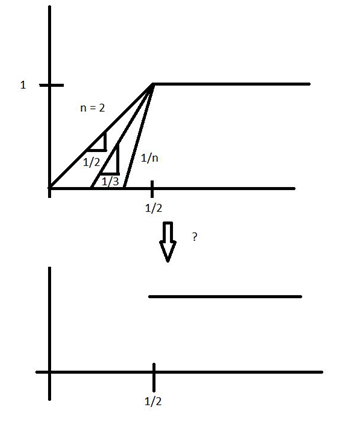
\includegraphics{graphics/Chap06/typeset.png}
        }
\caption[]{Visually, the sequence of continuous functions $(f_n(t))_{n=2}^\infty$ appears to be converging to a step function, which is discontinuous. If that is true, we then have a Cauchy sequence in $(\mathcal{X}, \| \bullet \|_1)$ that does not have a limit in the set $\mathcal{X}$. }
    \label{fig:NonConvergentCauchySequence}
    \end{figure}

\begin{example} Let $ \mathcal{X} :=  \{f:[0,1] \to \real \ \vert \ \textnormal{f is continuous}\}$ and equip it with the one-norm, $ \| f \|_1 := \int_0^1 \vert f(\tau)\vert d\tau$. Define a sequence as follow, where each function piecewise  is linear and $n \ge 2$,
    $$f_n(t)=\begin{cases}
        0 & 0\leq t\leq\frac{1}{2}-\frac{1}{n}\\
        1+n(t-\frac{1}{2}) & \frac{1}{2}-\frac{1}{n}\leq t\leq\frac{1}{2}\\
        1 & t\geq\frac{1}{2}.
    \end{cases}
    $$
    \textbf{Show that the sequence is Cauchy and does not have a limit in $ \mathcal{X}$}.
 
 \end{example} 
 
 \textbf{Proof:}  You may want to check that each function is continuous at the breakpoints, $\frac{1}{2}-\frac{1}{n}$ and $\frac{1}{2}$. Moreover, by using the area under a triangle, you can show
    $\| f_n - f_m \|_1=\frac{1}{2}$  $|\frac{1}{n}- \frac{1}{m}|$ $\xrightarrow[n,\ m \to \infty]{ }0$, and thus the sequence is Cauchy. \\
    
    
How can we show that there does not exist any (continuous) function $f \in \mathcal{X}$ to which the sequence converges? We define 
 $$f_{\rm step}(t):= \begin{cases} 0 & 0 \le  t < \frac{1}{2} \\ 1 &  \frac{1}{2} \le t \le 1 \end{cases}$$
 and note that $f_{\rm step}$ is discontinuous and hence $f_{\rm step} \not \in \mathcal{X}$. Define $\mathcal{Y}:=\spanof{ \mathcal{X}, f_{\rm step}} \subset \{ f:[0, 1] : \real \}$, the vector space of all functions from the interval $[0, 1]$ to the real numbers. You can check that $\| \bullet \|_1$ is also a norm on $\mathcal{Y}$ and observe that $f\in \mathcal{Y}$ is continuous if, and only if, $f\in \mathcal{X}$. Finally, you can easily compute that
 $$\|f_n - f_{\rm step} \|_1=\frac{1}{2n},$$ 
 and hence, $f_n \to f_{\rm step}$. By uniqueness of limits, there does not exist a continuous function in $\mathcal{Y}$ to which the sequence converges, and thus the sequence does not have a limit in $\mathcal{X}$. 
 
 \Qed

The study of Cauchy sequences led mathematicians to wonder if it is possible to find normed spaces where all Cauchy sequences do have limits (within the given normed space), and moreover, if a normed space was ``deficient'' in the sense that it had Cauchy sequences without limit, could it be ``enlarged'' or ``completed'' to one where all Cauchy sequences do have limits. These are great questions!

\begin{definition} A normed space $(\mathcal{X},\real,\|\cdot\|)$ is \textbf{complete} if every Cauchy Sequence in $X$ has a limit in $X$. Such spaces are also called \textbf{ Banach spaces}.
\end{definition} 

The above definition can only be useful if a list of useful Banach spaces is known; see \url{https://en.wikipedia.org/wiki/Banach_space#Examples_2}.   In EECS562, you will use $\left(C\left[0,\ T\right],\ \| \bullet \|_\infty\right)$, the set of continuous functions with the infinity (or max) norm. The sequence in Fig.~\ref{fig:NonConvergentCauchySequence} is not a Cauchy sequence in $\left(C\left[0,\ T\right],\ \| \bullet \|_\infty\right)$; you might want to check that.

\begin{fact} For $a<b$, both finite, $(C\left[a,\ b\right]$, $\| \bullet \|_\infty)$ is complete where $C\left[a,\ b\right]=\left\{f:\left[a,\ b\right]\to\real\ |\ f\textnormal{ continuous}\right\}$. We showed above that $(C[a, b], ||\bullet||_1)$ is not complete.
\end{fact}


\begin{definition} A subset $S$ of a normed space is \textbf{ complete} if every Cauchy Sequence in $S$ has a limit in $S$.

\end{definition} 

\begin{rem} $S$ is complete implies that $S$ is closed.
    
\end{rem}

\begin{thm} Let $(\mathcal{X}, || \bullet ||)$ be a normed space. Then,

\begin{enumerate} 
       \renewcommand{\labelenumi}{(\alph{enumi})}
        \setlength{\itemsep}{.1cm}
        \item Every finite dimensional subspace is complete.
        \item Any closed subset of a complete set is also complete.
    \end{enumerate}
\end{thm}

\begin{fact} Every normed space $(\mathcal{X}, || \bullet ||_X)$ has a \textbf{``completion''}. A bit loosely stated, this means there is a complete normed space $(\mathcal{Y}, || \bullet ||_Y)$ such that
\begin{enumerate}
       \renewcommand{\labelenumi}{(\alph{enumi})}
        \setlength{\itemsep}{.1cm}
    \item $\mathcal{X} \subset \mathcal{Y}$ ($\mathcal{X}$ can naturally be viewed as a subset of $\mathcal{Y}$. The precise definition involves isometric isomorphisms.)
    \item $\forall x\in \mathcal{X}$, $||x||_Y = ||x||_X.$ 
    \item $\overline{\mathcal{X}} = \mathcal{Y}$ ($\overline{\mathcal{X}}$ is the closure of $\mathcal{X}$ in $\mathcal{Y}$. Hence, $\mathcal{X}$ fits ``tightly'' into $\mathcal{Y}$ in that sense that for any point in $y \in \mathcal{Y}$, $d(y, \mathcal{X})=0$).
    \item $\mathcal{Y}$ = $\mathcal{X} \cup\{ \text{limit points of Cauchy sequences in } \mathcal{X}\}$
\end{enumerate}

\end{fact}

You might ask about the completion of $C[a,b]$ when the $||\bullet||_1$ is used? It turns out to be the set of Lebesgue integrable functions on $[0,1]$. We alluded to Lebesgue back in Chapter~\ref{sec:ProbableApology}.
    

\section{Contraction Mapping Theorem}
\label{sec:Contraction}

\begin{definition}
 Let $S \subset \mathcal{X}$ be a subset of a normed space $(\mathcal{X}, \| \bullet \|)$. A function $T : S \to S$ is a \textbf{ contraction mapping} if,
$ \exists ~0 \leq c < 1$ such that $\forall x,y \in S,$ 
$$ \|T\left(x\right)-T\left(y\right)  \| \leq c \|x-y\|.$$ 
A point $x^\ast \in S$ is a \textbf{fixed point} of $T$ if $T(x^\ast) = x^\ast$.
\end{definition}


\begin{thm}\textbf{(Contraction Mapping Theorem)} ~ If $T$ is a contraction mapping on a complete subset $S$ of a normed space $\left(\mathcal{X},\real,\| \bullet \|\right)$, then there exists a unique vector $x^\ast \in S$ such that $T\left(x^\ast\right) = x^\ast$. Moreover, for every initial point $x_0 \in S$, the sequence $x_{n+1} = T\left(x_n\right), n \geq 0$, is Cauchy, and $x_n \to x^\ast$.
\end{thm}

\textbf{ Proof:}~ Let $(x_n)$ be defined as in the statement of the theorem. Because $T$ is a contraction mapping, there exists $0 \le c < 1$ such that, for all $n\geq 1$,
    \begin{align*}
        \| x_{n+1}-x_n \| &= \| T\left(x_n\right)-T\left(x_{n-1}\right) \|\\
        &\leq c \| x_n-x_{n-1}\|
    \end{align*}
    
\begin{claim} $(x_n)$ is Cauchy and thus by the completeness of $S$, $\exists x^\ast \in S$ such that $x_n \to x^\ast$.
\end{claim} 

\textbf{Proof:} We leave as an exercise to show by induction that $\| x_{n+1}-x_n \| \leq c ^n\| x_1-x_0 \|$. Next, consider $\| x_m-x_n \|$, and without loss of generality, suppose $m=n+k,\ k > 0$. Then,
    \begin{align*}
        \| x_m-x_n \| &= \| x_{n+k}-x_n \|\\
        &= \| x_{n+k}-x_{n+k-1}+x_{n+k-1}- \dots +x_{n+1}-x_n\|\\
        &\leq \| x_{n+k}-x_{n+k-1}\|+ \dots + \| x_{n+1}-x_n\|\\
        &\leq \left(c ^{n+k-1}+c ^{n+k-2}+ \dots + c ^n\right)\|x_1-x_0\|\\
        &= c ^n \left( \sum\limits_{i=0}^{k-1} c ^i \right) \|x_1-x_0\|\\
        &\leq c ^n \left( \sum\limits_{i=0}^\infty c ^i \right)\|x_1-x_0\|\\
        &= \frac{c ^n}{1-c}\|x_1-x_0\| \xrightarrow[\substack{n\to \infty \\ m >n}]{}0
    \end{align*}
where we used a simple fact about the geometric series for $\frac{1}{1-c}$. Therefore, $\left(x_n\right)$ is Cauchy sequence in $S$, and by completeness, $\exists x^\ast \in S$ such that $x_n \to x^\ast$. 
$\hfill \square$

\begin{claim} $x^\ast=T\left(x^\ast\right)$ and thus $x^\ast$ is a fixed point of $T$.
\end{claim} 

\textbf{Proof:} Let $n\ge 1$ be arbitary. Then,
    \begin{align*}
        \| x^\ast-T\left(x^\ast\right) \| &= \| x^\ast-x_n+x_n- T\left(x^\ast\right)\| \\
        &=\| x^\ast-x_n+T\left(x_{n-1}\right)- T\left(x^\ast\right)\| \\
        &\leq \| x^\ast-x_n\|+\|T\left(x_{n-1}\right)- T\left(x^\ast\right)\| \\
        &\leq \| x^\ast-x_n\|+c \|x_{n-1}-x^\ast\| \xrightarrow[n\to \infty]{}0.\ 
    \end{align*}
    
    $\hfill \square$
    
\begin{claim}  $x^\ast$ is unique.
\end{claim}

\textbf{Proof:}~ Suppose $y^\ast=T\left(y^\ast\right)$. Then,
    \begin{align*}
        \|x^\ast-y^\ast\|&=\|T\left(x^\ast\right)- T\left(y^\ast\right)\| \\
        &\leq c \|x^\ast-y^\ast\|.
    \end{align*}
    The only non-negative real number $\gamma $ that satisfies $\gamma \le \gamma c$ for some $0 \le \c < 1$ is $\gamma=0$. Hence, due to the property of norms, $0=\|x^\ast-y^\ast\|\implies x^\ast=y^\ast$. 
    
    $\hfill \square$
    
    \Qed
    
\begin{rem} The (local) convergence of the Newton-Raphson Algorithm is accomplished by identifying a closed ball in $\real^n$ on which the function
 $$\boxed{T(x):= x-\epsilon\left(\pardiff[f]{x}(x)\right)^{-1}(f(x)-y)}$$
 is a contraction mapping. The estimate of a suitable value $0 \le c < 1$ is based on a Lipschitz constant for the Jacobian. We check that 
a solution of $f(x)-y$ is a fixed point of $T(x)$.
Indeed,
\begin{align*}
x^\ast & = T(x^\ast) \\
&\Updownarrow \\
x^\ast&=x^\ast-\epsilon\left(\pardiff[f]{x}(x^\ast)\right)^{-1}(f(x^\ast)-y)\\
&\Updownarrow \\
0&=-\epsilon\left(\pardiff[f]{x}(x^\ast)\right)^{-1}(f(x^\ast)-y)\\
&\Updownarrow \\
0&=(f(x^\ast)-y).
\end{align*}
\end{rem}
  

\section{Continuous Functions}

\begin{figure}[hbt!]%
	\centering{
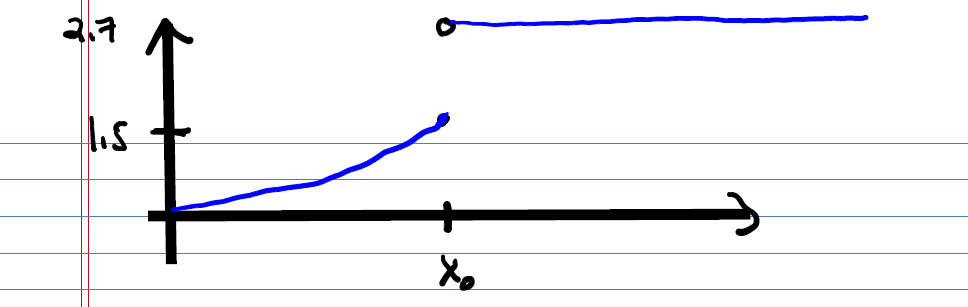
\includegraphics[width=0.7\columnwidth]{graphics/Chap06/Discontinuousfunction.png} }
    \caption[]{Let $\epsilon=1.0$ Then, $\forall~\delta>0, \exists~x\in B_\delta(x_0)$ such that $|f(x) - f(x_0)| \ge \epsilon$. Indeed, $x=x_0 +\delta_2$ works. }
    \label{fig:DiscontFunction}
\end{figure} 

\begin{definition} Let $\left(\mathcal{X},\| \bullet \|\right)$, and $\left(\mathcal{Y},||| \bullet |||\right)$ be normed spaces.
\begin{enumerate}
       \renewcommand{\labelenumi}{(\alph{enumi})}
        \setlength{\itemsep}{.1cm}
    \item $f:\mathcal{X} \to \mathcal{Y}$ is \textbf{ continuous at $x_0 \in \mathcal{X}$} if $\forall \epsilon > 0,~ \exists  \delta \left(\epsilon, x_0\right) > 0$ such that $ \|x-x_0\| < \delta \implies ||| f\left(x)\right) ||| < \epsilon.$
    
     \item $f$ is \textbf{ continuous} if it is continuous at $x_0$ for all $x_0 \in \mathcal{X}$.
 
\end{enumerate}

\end{definition} 

\begin{rem}
 It is also common to define continuity at a point as as $\forall ~\epsilon>0$, $\exists \delta>0$ such that $ x \in B_{\delta}\left(x_0\right) \implies  f\left(x\right) \in B_{\epsilon}\left(f\left( x_0\right)\right)$. Though less common, it can also be defined as $\forall ~\epsilon>0$, $\exists \delta>0$ such that $ f(B_{\delta}\left(x_0\right)) \subset  B_\epsilon(f(x_0))$.
\end{rem}

\begin{rem} \textbf{(Discontinuous at a point)} Let's negate the definition of $f$ continuous at $x_0$. $f$ is \textbf{discontinuous} at $x_0 \in \mathcal{X}$ if $\exists~\epsilon>0$ such that, $\forall~\delta >0, \exists ~x \in \mathcal{X}$ such that $||x-x_0||< \delta$ and $|||f(x) - f(x_0)||| \ge \epsilon$. This can also be stated as $\exists ~\epsilon>0$ such that, $\forall ~\delta>0$, $\exists~x \in B_\delta(x_0)$ such that $f(x) \not \in B_\epsilon(f(x_0))$. Finally, it can also be stated as $\exists ~\epsilon>0$, $\forall \delta>0$ such that $ f(B_{\delta}\left(x_0\right)) \not \subset  B_\epsilon(f(x_0))$.
\end{rem}

\begin{thm} \textbf{(Characterization of Continuity at a Point via Sequences)} Let  Let $\left(\mathcal{X},\| \bullet \|\right)$, and $\left(\mathcal{Y},||| \bullet |||\right)$ be normed spaces and $f:\mathcal{X} \to \mathcal{Y}$ a function.
    \begin{enumerate}
       \renewcommand{\labelenumi}{(\alph{enumi})}
        \setlength{\itemsep}{.1cm}
        \item If $f$ is continuous at $x_0$ and the sequence $\left(x_n\right)$ is a sequence in $\mathcal{X}$ that converges to $x_0$, then the sequence $(y_n:=f(x_n))$ in $\mathcal{Y}$ converges to $f(x_0)$. [$y_n:=f(x_n)$, $y_0:=f(x_0)$ implies $y_n \to y_0$ when $f$ is continuous at $x_0$. ]
        \item If $f$ is discontinuous at $x_0$, then there exists a sequence $\left(x_n\right)$ such that $ x_n \to x_0$, and $f\left(x_n\right) \not \to  f\left(x_0\right)$, that is, $f\left(x_n\right)$ does not converge to $f\left(x_0\right)$.
    \end{enumerate}
    
\end{thm} 

The proof is done in HW 10. The main point is, just as sequences can be used to completely characterize closed sets, they can also be used to completely characterize continuity at a point. 

\begin{cor} $f:\mathcal{X} \to \mathcal{Y}$ is continuous at $x_0$ if, and only if, every convergent sequence in $\mathcal{X}$ with limit $x_0$ is mapped by $f$ to a convergent sequence in $\mathcal{Y}$ with limit $f(x_0)$. In other symbols,  ($f$ is continuous at $x_0$)$\iff (x_n \to x_0 \implies f(x_n) \to f(x_0)).$ 

\end{cor}

\section{Compact Sets and the Existence of Extrema of Functions}

\begin{definition}  Let $(x_n)$ be a sequence and $1\le n_1<n_2<n_3<\dotsb $ be an infinite set of strictly increasing integers. Then, $(x_{n_i})$ is called a \textbf{ subsequence} of $(x_n)$. We note in passing that $n_i \ge i$, $\forall ~i\ge1$.
\end{definition}

\begin{example} $n_i = 2i + 1\textnormal{ or } n_i = 2^i.$
    
\end{example}

\begin{lem}
\label{lem:SubSequencesConverge}
 Suppose $x_n\to x$. Then every subsequence $(x_{n_i})$ of $(x_n)$ converges to $x$.
\end{lem}

We leave the proof as an exercise. 

\begin{definition} A set $S$ is \textbf{ bounded} if $\exists~ r < \infty$ such that $S \subset B_r(0)$.
\end{definition}

\begin{exercise} 
\label{exer:UnboundedStuff}
Show the following for $S\subset \mathcal{X}$:
\begin{enumerate}
    \item $S$ is bounded if, and only if, $\sup_{x\in S} \| x \| < \infty$.
     \item Hence, $S$ is unbounded if, and only if, $\sup_{x\in S} \| x \| = \infty$.
    \item $S$ is unbounded if, and only if, there exists a sequence $(x_k)$ such that, for all $k\ge 1$, $x_k\in S$ and $||x_{k+1}||\ge ||x_k|| + 1$.
\end{enumerate}
\end{exercise}

\begin{lem} If $S$ is unbounded, then it contains a sequence with no convergent subsequence.
\end{lem}

\textbf{Proof:} The sequence $(x_n)$ constructed above in Exercise~\ref{exer:UnboundedStuff} has no convergent subsequence. Indeed, by Remark~\ref{rem:HandyInequality}, if $(x_{n_i})$ is a subsequence of $(x_n)$, then $\| x_{n_i} -x_{n_j}\| \ge | ~\| x_{n_i}\| - \|x_{n_j}\|~| \ge |n_i - n_j|$, and thus is not Cauchy. Because it is not Cauchy, it cannot be convergent.

\Qed 

\begin{definition} \textbf{(Equivalent Norms)} Let $({\cal X}, \real)$ be a vector space. Two norms $||\cdot||:{\cal X} \to[0, \infty)$ and $|||\cdot|||:{\cal X} \to [0, \infty)$ are \textbf{equivalent} if there exist positive constants $K_1$ and $K_2$ such that, for all $x\in {\cal X}$,
    $$K_1 |||x||| \le ||x|| \le K_2 |||x|||. $$
\end{definition} 

\begin{rem}
It follows from the definition of equivalent norms that
$ \frac{1}{K_2}||x|| \le |||x||| \le \frac{1}{K_1} ||x||. $  
\end{rem}
-

We'll next develop a few bounds for norms on finite dimensional vector spaces, and use the bounds to relate convergence of a sequence of vectors in a finite dimensional normed space $(\mathcal{X}, ||\bullet ||)$ to the convergence of the representation of the sequence with respect to a basis. Let $\{v\}:=\{v^1, v^2, \ldots, v^n \}$ be a basis for $\mathcal{X}$ and define $M_i :=\spanof{v^j~| j \neq i}$, the $(n-1)$-dimensional subspace spanned by all the basis vectors except the $i$-th one. Because $M_i$ is finite dimensional, it is a complete and hence a closed subset of $\mathcal{X}$. By construction, $v^i \not \in M_i$, and thus, 
$$\delta_i:= d(v^i, M_i)>0. $$

\begin{lem} Let $\{v\}=\{v^1, v^2, \ldots, v^n \}$, $\{M_1, M_2, \ldots, M_n\}$ and $\{\delta_1, \delta_2, \ldots, \delta_n\}$ be as above. Then for any vector $x = \alpha_1 v^1+ \alpha_2 v^2 + \cdots + \alpha_n v^n \in \mathcal{X}$, 
\begin{equation}
\label{eq:equivalentNormsWithRepresentations}
    \kappa_\ast \left( \max_{1 \le i \le n} |\alpha_i| \right)  \le  ||x|| \le \kappa^\ast \left( \sum_{i=1}^n |\alpha_i| \right) \le n \kappa^\ast  \left( \max_{1 \le i \le n} |\alpha_i| \right),
\end{equation} 
where $\kappa_\ast:=\min_{1 \le i \le n}\{ \delta_i\}>0$, $\kappa^\ast := \max_{1 \le i \le n}\{ ||v^i||\} < \infty$, and $\alpha:=[x]_{\{v\}}$.

\end{lem}

\textbf{Proof:} The right hand side of \eqref{eq:equivalentNormsWithRepresentations} follows from the triangle inequality for norms. The proof of the left hand side of \eqref{eq:equivalentNormsWithRepresentations} requires a few steps that we carefully enumerate and leave to the reader:
\begin{enumerate}
    \item If $\alpha_i=0$, then $d(\alpha_i v^i, M_i) =0$. 
    \item If  $\alpha_i\neq 0$, then $d(\alpha_i v^i, M_i) = |\alpha_i|d(v^i, M_i) = |\alpha_i| \delta_i$.
    \item Hence, for all $\alpha_i \in \real$, $d(\alpha_i v^i, M_i) = |\alpha_i| \delta_i$
    \item For arbitrary $m_i \in M_i$, $d(\alpha_i v^i+m_i, M_i)=d(\alpha_i v^i-m_i, M_i)=d(\alpha_i v^i, M_i).$
    \item For any vector $x = \alpha_1 v^1+ \alpha_2 v^2 + \cdots + \alpha_n v^n \in \mathcal{X}$, $d(x, M_i) = d(\alpha_i v^i, M_i)$.
    \item Hence for any vector $x = \alpha_1 v^1+ \alpha_2 v^2 + \cdots + \alpha_n v^n \in \mathcal{X}$, and for all $1 \le i \le n$,
    $$||x|| \ge \inf_{m \in M_i} || x - m|| =: d(x, M_i) = |\alpha_i| \delta_i.$$
\end{enumerate}
\Qed

\begin{cor} \textbf{(Equivalent Norms)} All norms on finite dimensional vector spaces are equivalent\footnote{It is an interesting fact that a vector space is finite dimensional if, and only if, all norms on it are equivalent.}.
\end{cor}

\textbf{Proof:} Equation~\eqref{eq:equivalentNormsWithRepresentations} shows that, once a basis is chosen, any norm on an $n$-dimensional normed space is equivalent to $(\real^n, ||\bullet||_{\rm max})$. We leave it to the reader to show that this is enough to prove the result. 
\Qed

\begin{cor} \textbf{(Convergence of Components of Sequences in Finite-dimensional Spaces)}
\label{cor:Reduce2Reals}
Let $(x_k)$ be a sequence in a finite dimensional normed space $(\mathcal{X}, ||  \bullet ||)$ with basis $\{v^1, v^2, \ldots, v^n \}$. Let $$\mathbf{\alpha}_k:=[x_k]_{\{v\}} \in \real^n$$
be the representation of $x_k$ with respect to the basis $\{v\}$ so that 
$x_k =  \mathbf{\alpha}_{k,1} v^1+ \mathbf{\alpha}_{k,2} v^2 + \cdots + \mathbf{\alpha}_{k,n} v^n. $ Then $(x_k)$ is a Cauchy sequence in $\mathcal{X}$ if, and only if, each sequence $(\mathbf{\alpha}_{k,i})$ is a Cauchy sequence in $(\real, |\bullet |)$, $1 \le i \le n$.
\end{cor}

\textbf{Proof:} Equation~\eqref{eq:equivalentNormsWithRepresentations} reduces the proof to understanding that a sequence in $\real^n$ is Cauchy if, and only if, each of its real components is Cauchy. But with the max-norm, $(\real^n, ||\bullet||_{\rm max})$, this is quite easy to show because it selects the largest element, and if the largest element is getting small, then the rest of them are too. Have fun with it! 
\Qed

\begin{figure}[hbt!]%
	\centering{
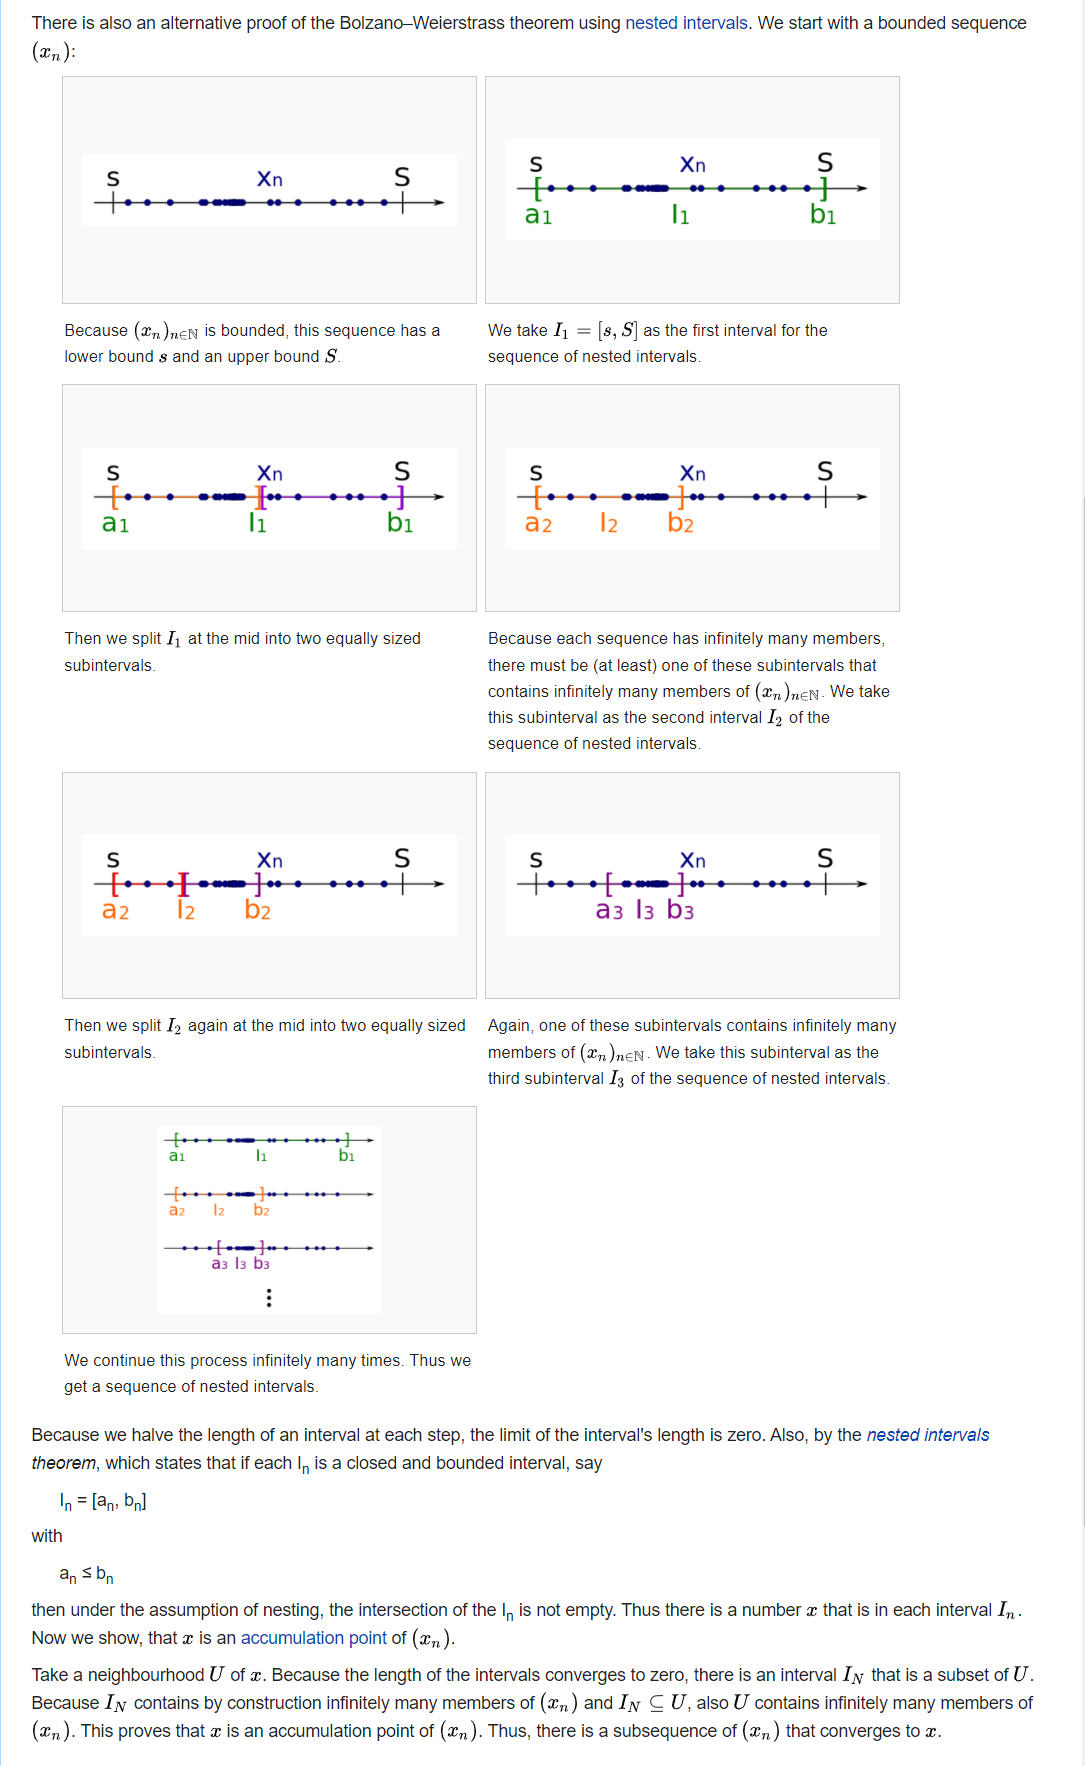
\includegraphics[width=0.72\columnwidth]{graphics/Chap06/BolzanoWeirstrassNestedIntervals.png} 
}
    \caption[]{ Illustration of a sequntial comactness proof from Wikipedia \url{https://en.wikipedia.org/wiki/Bolzano-Weierstrass_theorem}.}
    \label{fig:BolzanoWeirstrassProof}
\end{figure} 


\begin{thm} 
\label{thm:BolWeir}
\textbf{(Bolzano-Weierstrass Theorem or the Sequential Compactness Theorem)}~ In a finite dimensional normed space $(\mathcal{X}, ||  \bullet ||)$,
the following two properties are equivalent for a set $C \subset \mathcal{X}$.
\renewcommand{\labelenumi}{(\alph{enumi})}
\begin{enumerate}
\item $C$ is closed and bounded;
\item Every sequence in $C$ contains a convergent subsequence, that is, for every sequence $(x_n)$ in $C$ (i.e. $x_n \in C, \forall~n\ge 1$), there exists $x_0 \in C$ and a subsequence
$(x_{n_i})$ of $(x_n)$ such that $x_{n_i} \to x_0$.
\end{enumerate}
\end{thm}

\textbf{Proof:} We first show $\sim(a) \implies \sim (b)$. There are two cases, $C$ is not closed or $C$ is not bounded. \\

Suppose that $C$ is not closed. Then by Corollary~\ref{cor:ClosureAndLimitPoints}, there exists a limit point $x_0 \in \overline{C}$ such that $x_0 \not \in C$. Hence, there exists a sequence $(x_n)$ with $x_n \in C$ and $x_n \to x_0 \not \in C$. By Lemma~\ref{lem:SubSequencesConverge}, all subsequences $(x_{n_i})$ of $(x_n)$ satisfy $x_{n_i} \to x_0$. Hence, we have constructed a sequence of elements of $C$ for which there is no subsequence with a limit in $C$. \\

Suppose next that $C$ is unbounded. Then Exercise~\ref{exer:UnboundedStuff} produces a  sequence of elements of $C$ for which every subsequence is not Cauchy, and hence cannot have a limit in $C$. This completes the proof of $\sim(a) \implies \sim (b)$. Nothing we have done so far depends on $\mathcal{X}$ being finite dimensional.\\

We now turn to $(a) \implies (b)$. Let $(x_n)$ be an arbitrary sequence built from elements of $C$. To show: it has a convergent subsequence with limit in $C$.\\

\ul{Case 1:}  $(x_n)$ has only a finite number of distinct elements. Hence, at least one value is repeated an infinite number of times; let's call it $x_N \in C$. Because it is repeated an infinite number of times, we can choose a strictly increasing sequence $n_1 < n_2 < \cdots < n_i < \cdots$ such that $x_{n_i}=x_N$ for all $i \ge 1$. The subsequence $(x_{n_i})$ converges to $x_N \in C$ and hence we are done.\\

\ul{Case 2:} $(x_n)$ has an infinite number of distinct elements. Here, we will invoke that $\mathcal{X}$ is finite dimensional. Indeed, by Corollary~\ref{cor:Reduce2Reals}, a subsequence of $(x_n)$ will be convergent if, and only if, once it it is represented with respect to a basis, each of its components is convergent. Hence, it is enough to prove that every real sequence $(a_n)$, with an infinite number of distinct elements, contained in a closed and bounded subset of $C_1 \subset \real$ has a convergent subsequence. Every bounded subset of $\real$ is contained within a closed interval of the form $[-N, N]$, for some integer $1 \ge N < \infty$, and hence we reduce ourselves to a set $C_1 \subset [-N, N]$ and $C_1$ contains an infinite number of (distinct) elements of the sequence $(a_n)$. Because $C_1$ contains an infinite number of distinct elements of $(a_n)$, some closed interval of the form $[n, n+1]$, for $|n|\le N$ must contain an infinite number of elements of $(a_n)$. Without loss of generality, we will assume the closed interval $[0, 1]$ contains an infinite number of elements of $(a_n)$; the reader will see that our argument works \emph{mutatis mutandis} for any other interval of length one.\\

Divide the interval $[0, 1]$ into two halves, $[0, 1] = [0, 1/2] \cup [1/2, 1]$. At least one of the halves must contain an infinite number of elements of $(a_n)$. For the sake of argument, assume it is the right half. Now we divide in half $[1/2, 1] = [1/2, 3/4] \cup [3/4, 1]$ and note that at least one of the halves must contain an infinite number of elements of the sequence $(a_n)$. For the sake of argument, assume the left half this time. We then divide in half $[1/2, 3/4]=[1/2, 5/8] \cup [5/8, 3/4]$  and note that at least one of the halves must contain an infinite number of elements of the sequence $(a_n)$.\\

At the $k$-th step, we have a closed sub-interval of $I_k \subset [0, 1]$, with length $I_k$ equalling $1/2^k$ and $I_k$ contains an infinite number of distinct elements of $(a_k)$. Hence, for all $k\ge 1$, there exists $n_k$ such that $n_k > n_{k-1}$ and $a_{n_k} \in I_k$. Moreover, the sequence $(a_{n_k})$ is Cauchy because for all $i\ge k, j \ge k$, $|a_{n_i}- a_{n_j}| \le 1/2^k$. Hence the subsequence $(a_{n_k})$ converges to a limit in $C_1$ and the proof is done.

\Qed


\begin{definition} A set $C$ satisfying (a) or (b) of Theorem~\ref{thm:BolWeir} is said to be \textbf{ compact}. 
\end{definition}.


\begin{rem}
There are various definitions of compactness that are appropriate for specific settings. The one above is typically called sequential compactness. Because it is the only form of compactness we use in these notes, we will drop the term sequential and simply call such sets compact sets. 
\end{rem}


\begin{thm} \textbf{(Weierstrass Theorem)}~ If $C$ is compact and $f: C \to \real$ is continuous, then $f$ achieves its extreme values. That is,
    \begin{equation*}
        \exists x^\ast \in C\textnormal{, s.t. }f(x^\ast)=\sup\limits_{x\in C}f(x)
    \end{equation*}
    and
    \begin{equation*}
        \exists x_* \in C\textnormal{, s.t. }f(x_*)=\inf\limits_{x\in C}f(x).
    \end{equation*}

\end{thm}

\textbf{Proof:}~ Let $f^\ast:=\sup\limits_{x\in C}f(x)$. To show $\exists x^\ast \in C$, such that $f(x^\ast)=f^\ast$.\\

\begin{claim} $f^\ast$ is finite.
\end{claim}

{Proof:} We do a proof by contradiction and suppose not, that is, suppose $f^\ast = \infty$. Then, by definition of the supremum, for all $n\ge 1$, there exists $x_n \in C$ such that $f(x_n) \ge n$. Because $C$ is compact, there exists $x_0 \in C$ and a subsequence $(x_{n_i})$ of $(x_n)$ such that
$x_{n_i} \to x_0$. Because $f$ is assumed continuous, 
$$f(x_0) = \lim_{i \to \infty} f(x_{n_i}) \ge   \lim_{i \to \infty} n_i = \infty.$$
But because $f:C \to \real$, $f(x_0) \in \real$, which contradicts $f(x_0) = \infty$. Hence, it cannot be the case that $f^\ast = \infty$.

$\hfill \square$

Continuing with the proof, we now know that $f^\ast$ is finite. Once again, applying the definition of the supremum, we have that $\forall n>0, \exists ~x_n\in C$ such that $|f^\ast-f(x_n) |<1/n$. Because
    $C$ is compact,  there exists $x^\ast \in C$ and a subsequence $(x_{n_i})$ such that 	$x_{n_i} \to x^\ast$. Because $f$ continuous, $f(x_{n_i})\to f(x^\ast)$. We expect to show that $f(x^\ast) = f^\ast$. To do so, we note that, by the continuity\footnote{Technically, we are using the continuity of $f$ implies that of $g(x):=|f^\ast - f(x)|$, which you are welcome to check. Otherwise, you can do the estimate as $|f^\ast -f(x^\ast)| =|f^\ast - f(x_{n_i}) + f(x_{n_i})- f(x^\ast)| \le  |f^\ast - f(x_{n_i})| + |f(x_{n_i}) - f(x^\ast)|  \le \frac{1}{n_i} + |f(x_{n_i}) - f(x^\ast)|  \xrightarrow[i\to \infty]{}0.$ } of $f$,
$$|f^\ast -f(x^\ast)|= \lim_{i \to \infty} |f^\ast - f(x_{n_i})|  \le  \lim_{i \to \infty} \frac{1}{n_i}=0. $$
And hence, 
    $f^\ast=f(x^\ast)$.\\
    
    The same proof works for the infimum. 
    
    \Qed

